\chapter{Aufbereitung der 3D-CAD Daten}
\label{sec:AufbereitungDer3D-CADDaten}

\section{Eine kurze Einführung zum Aufbau von 3D-Objekten}
\label{sec:KurzerEinschubZumAufbauVon3D-Objekten}

\begin{wrapfigure}{R}{0.5\textwidth}
	\centering
	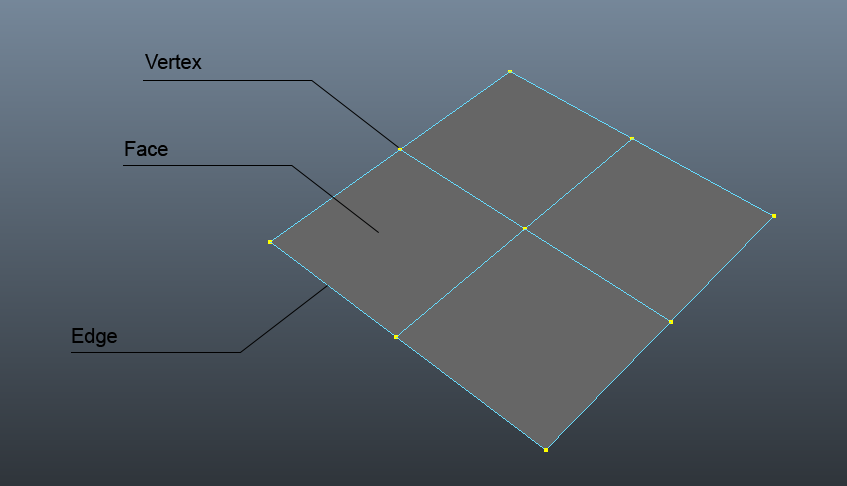
\includegraphics[width=0.5\textwidth]{bildquellen/face_edge_vertex}
	\caption{Eine Plane, bestehend aus vier quadratischen Polygonen.}
\end{wrapfigure}
In gängigen 3D-Programmen geschieht die Modellierung mit Hilfe von polygonalen Netzen (oder Meshes), welche in der 3D-Computergrafik häufig anzutreffen sind. Polygonnetze, also Netze die sich aus einer Menge von miteinander verbundenen Polygonen zusammensetzen, bestehen zumeist aus Dreiecken und Vierecken. Es lassen sich damit einfache geometrische Figuren wie Zylinder, Kugeln, Prismen, Würfel, Tetraeder, Pyramiden etc., aber auch komplexere Strukturen erschaffen, um bspw. Modelle für Computerspiele oder Animationsfilme zu erstellen.\footnote{Vgl. Michael Bender, Manfred Brill (2006): \textit{Computergrafik}. 2.Aufl. München: \newline Carl Hanser Verlag. S. 19.}

In Autodesk Maya werden polygonale Flächen auch als Faces bezeichnet und haben drei oder mehr begrenzende Kanten, die Edges genannt werden. Die Edges wiederum sind über Punkte, den sogenannten Vertices (Plural) miteinander verbunden. Diese drei formgebenden Elemente können transformiert werden, um ein polygonales Netz zu deformieren. Genutzt werden dafür die verschiedenen Transform-Attribute, Translation, Rotation und Skalierung.\footnote{Vgl. Todd Palamer (2014): \textit{Vgl. Mastering Autodesk Maya 2015}. 1.Aufl. Indianapolis: Sybex. S. 107 f.} Zusätzlich können weitere Unterteilungen eingesetzt werden, um ein Polygonnetz feiner zu strukturieren. Es ist möglich Faces, Edges und Vertices miteinander zu verbinden, aufzutrennen oder um jeweils neue Elemente zu erweitern (extrudieren). 

\section{Analyse des CAD-Exports}
\label{sec:AnalyseDesCAD-Exports}
Bevor das aus CAD exportierte Modell in Unity importiert wird, sollte selbiges vorher in einem geeigneten 3D-Programm überprüft werden. Für diesen Zweck wird, wie im vorangegangenen Abschnitt erwähnt auf Autodesk Maya zurückgegriffen. Maya ist eine professionelle Software für Modellierung, Animation und Rendering von 3D-Objekten und Szenen.\footnote{Vgl. Autodesk  (2018): \textit{MAYA}.\newline
\url{https://www.autodesk.de/products/maya/overview},\newline 
abgerufen am 30.08.2018.}

\begin{figure}[H]
	\centering
	\captionsetup{width=1\textwidth}
	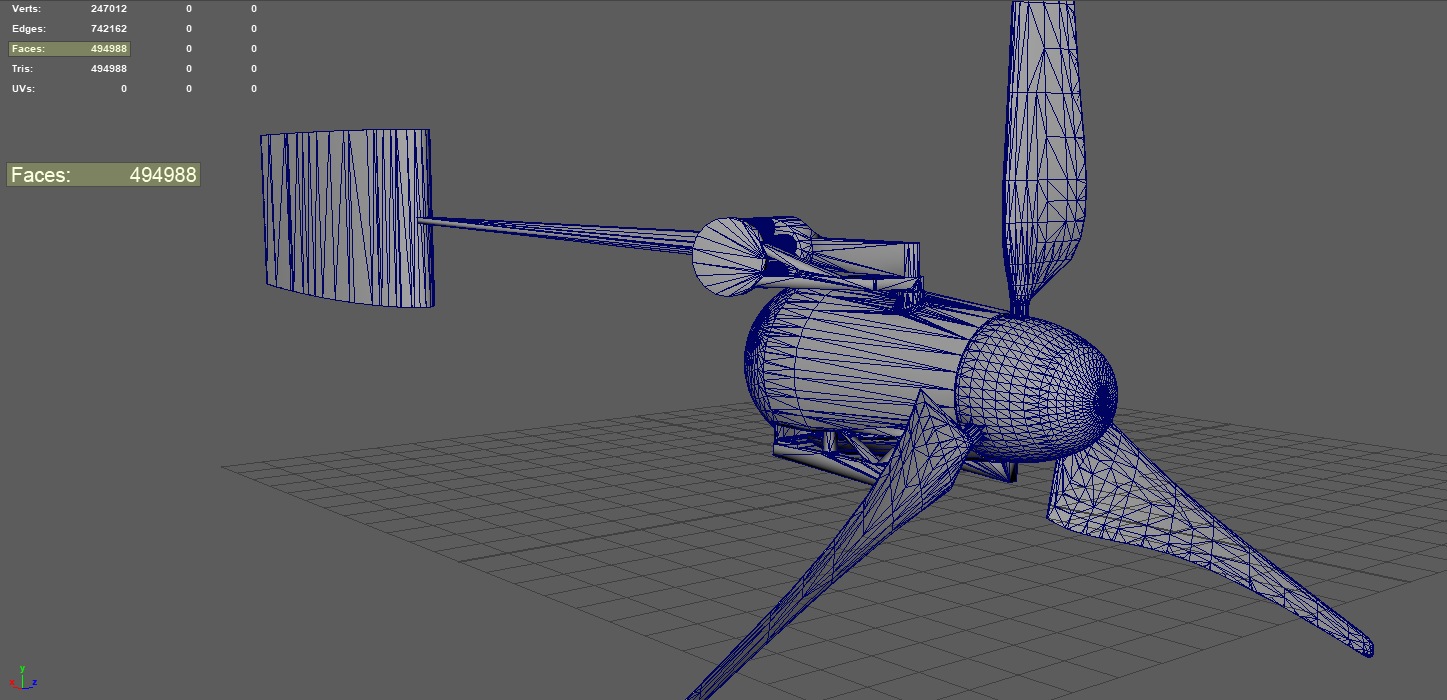
\includegraphics[keepaspectratio, width=1\textwidth]{bildquellen/WEA-Vergleich1}
	\caption{Ergebnis des Exportes der WEA aus der CAD-Anwendung bestehend aus 494.988 Polygonen.}
	\label{fig:2.2}
\end{figure}

Das importierte Modell \sieheAbb{2.1} weist mehrere Eigenschaften auf, welche es für einen Import sowie eine Weiterverarbeitung in Unity ungeeignet machen. Die betreffenden Eigenschaften sind nachfolgend aufgelistet. 
Generell sollten Modelle mit möglichst wenigen Polygonen auskommen, da ein hoher Detailgrad über Texturen generiert werden kann. Im Falle einer technischen Darstellung die neben der äußeren Verkleidung auch innenliegende technische Baugruppen wie Wälzlager, Getriebe o.Ä. abbildet, kann dass die Anzahl der Polygone deutlich erhöhen. Schließlich müssen diese in adäquater Qualität dargestellt werden. Natürlich gilt aber auch hier der Grundsatz, dass eine zu geringe Anzahl zu lasten der Darstellungsqualität und eine zu hohe Anzahl zu lasten der Performance geht. Es gilt also einen guten Mittelweg zu finden. 


\begin{itemize}
\item \textbf{Polygon Count:} Das Modell besteht aus nicht ganz 500.000 Polygonen, was für eine Echtzeitanwendung sehr viel ist. Laut der Unity Dokumentation sollte der Polygon Count vom Zielsystem und der angestrebten Qualität abhängig sein. Das Optimum liegt für Desktopanwendungen bei 1500 bis 4000 Polygonen pro Objekt. Falls sehr viele Objekte zur selben Zeit aktiv sind, wird eine Reduktion der Polygone empfohlen.\footnote{Vgl. Unity Documentation  (2018): \textit{Modeling characters for optimal performance}.\newline
\url{https://docs.unity3d.com/Manual/ModelingOptimizedCharacters.html},\newline 
abgerufen am 30.08.2018.} Eine Empfehlung für eine maximale Beschränkung wird aber nicht gegeben.      

\item \textbf{Unterteilung in Einzelobjekte:} Die WEA setzt sich aus vielen Einzelobjekten zusammen. Diese sind vom größten Rotorblatt bis zur kleinsten Schraube zu einem einzigen Objekt zusammengefasst. Es ist also nicht möglich einzelne Teilobjekte in Unity separat mit Materialien und Skripten auszustatten oder zu animieren.  

\item \textbf{Flächenverteilung:} Ferner führt die ungleichmäßige Flächenverteilung im STL-Export zu Darstellungsfehlern beim Shading \sieheAbb{2.2}. Eng zusammenliegende Edges beeinflussen das visuelle Endergebnis negativ.
\end{itemize}

\begin{figure}[H]
	\centering
	\captionsetup{width=1\textwidth}
	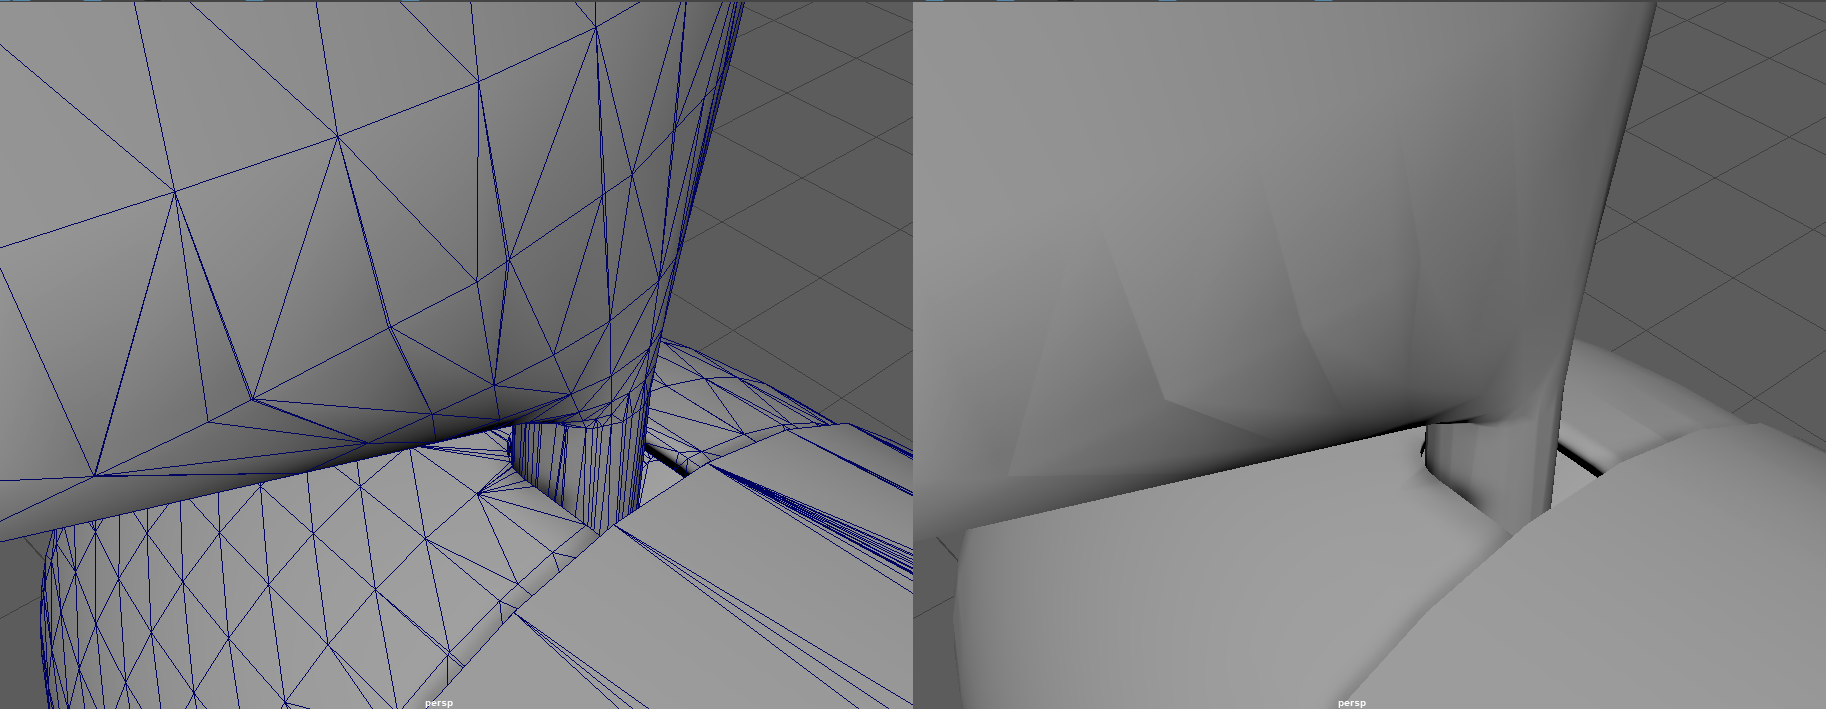
\includegraphics[keepaspectratio, width=1\textwidth]{bildquellen/WEAfehlerhaftesshading}
	\caption{Shadingfehler am Exportmodell.}
	\label{fig:2.3}
\end{figure}

Um diese Probleme zu lösen ist eine Retopologisierung, also eine Überarbeitung der geometrischen Grundstruktur und eine damit einhergehende Reduktion der Flächen nötig. Diese Vorgehensweise wird im folgenden Kapitel \sieheKapitel{\hyperref[sec:RetopologisierungDesCAD-Exports]{3.3 Retopologisierung des CAD-Exports}} beschrieben.

\label{sec:RetopologisierungDesCAD-Exports}
\section{Retopologisierung des CAD-Exports}
Die Aufbereitung des Modells kann händisch oder automatisiert erfolgen. Die händische Retopologisierung ist aufwändiger und erfordert Kenntnisse in der Polygonmodellierung. Die Qualität und die Anzahl der Polygone des Modells können aber exakt gesteuert werden. Eine automatische Reduktion hat aufgrund von invalider Geometrie, sogenannter non-manifold geometry aber nicht funktioniert. Das folgende Zitat aus der Maya LT Dokumentation von Autodesk beschreibt in Kürze das Problem. 

\begin{quote}
\glqq Some types of polygon geometry will not work in Maya. Invalid geometry includes vertices that are not associated with a polygon edge and polygon edges that are not part of a face (dangling edges). While Maya does not let \clearpage
 you create these types of geometry, it may be possible to import these types from other software applications.\grqq\footnote{Autodesk  (2015): \textit{Two-manifold vs. non-manifold polygonal geometry}.\newline\href{https://knowledge.autodesk.com/support/maya-lt/learn-explore/caas/CloudHelp/cloudhelp/2015/ENU/MayaLT/files/Polygons-overview-Twomanifold-vs--nonmanifold-polygonal-geometry-htm.html}{https://knowledge.autodesk.com/support/maya-lt/\dots},\newline abgerufen am 05.09.2018.} 
\end{quote}

Der Import aus CAD enthielt diese invalide Geometrie. Bei einem solch komplexen Modell eine Fehlersuche einzuleiten ist aber sehr zeitaufwendig und das Ergebnis der Autoreduktion ist qualitativ minderwertig, wie die folgende Abbildung aus einem anderen Projekt zeigt \sieheAbb{2.4}. 

\begin{figure}[H]
	\centering
	\captionsetup{width=0.8\textwidth}
	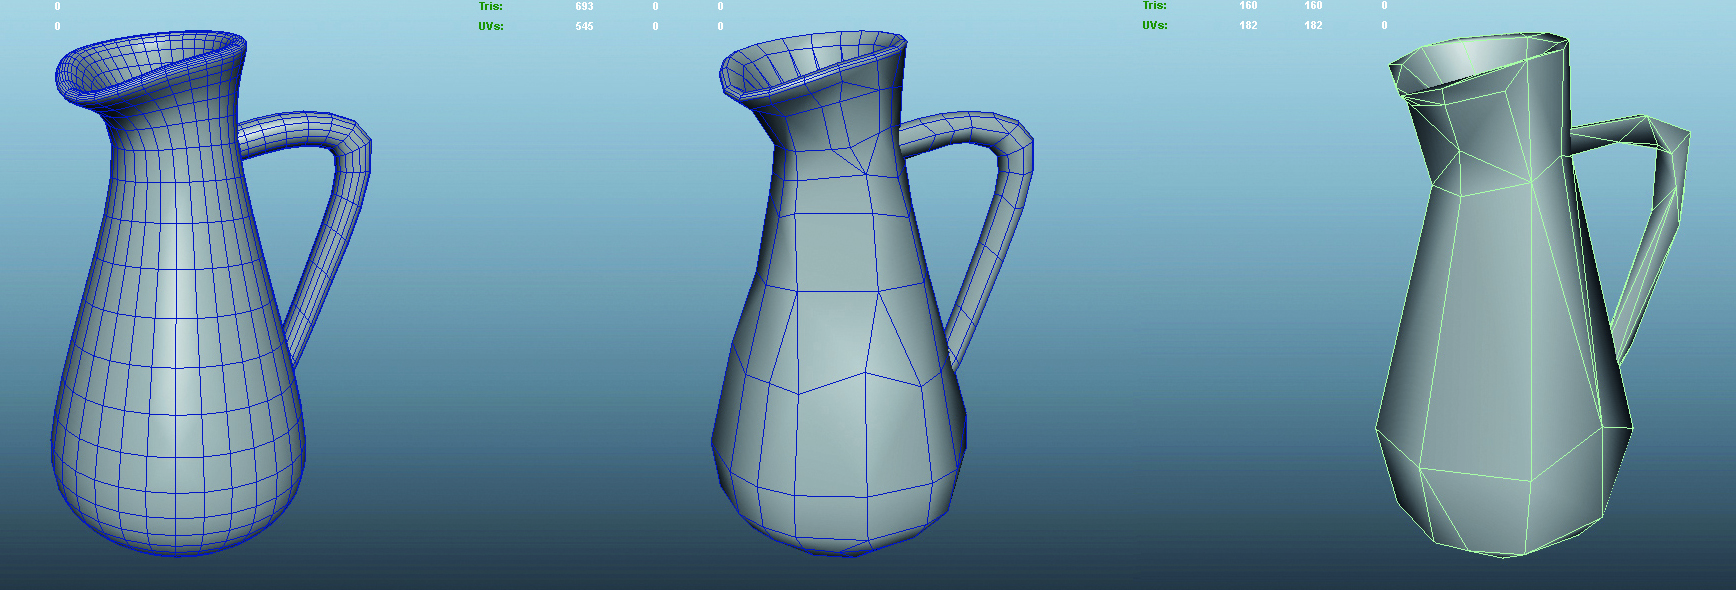
\includegraphics[keepaspectratio, width=0.8\textwidth]{bildquellen/hp-zu-lp-automatisch}
	\caption{Automatische Reduktion der Polygone auf (v.l.n.r.) 1536, 382 und 117.}
	\label{fig:2.4}
\end{figure}

Daher erschien es praktikabler das Modell händisch aufzubereiten. Die Aufbereitung erfolgte in Maya anhand von Polygonmodellierung, auf Basis von primitiven Körpern (Primitives). Das können bspw. Würfel, Zylinder, Kugeln, Tori etc. sein.  Mit Erzeugung dieser Primitives lässt sich durch Flächenextrusion die grobe Form nachbauen und mit Hilfe weiterer Unterteilungen verfeinern. Diese Anpassung des Primitives an die Form des CAD-Exportes geschieht für alle drei Raumdimensionen. Um eine sehr genaue Abbildung zu erzeugen können die Vertices des erzeugten Primitives an die Vertices des CAD-Modells \glqq angedockt\grqq\, werden. Es ist mit wenigen Werkzeugen möglich eine Abbildung des ursprünglichen Objektes mit guter Topologie und einer deutlich reduzierten Anzahl an Polygonen zu erzeugen. Die Vorgehensweise wird nachfolgend anhand eines Beispiels verdeutlicht \sieheAbb{2.5}.

\begin{figure}[H]
	\centering
	\captionsetup{width=1\textwidth}
	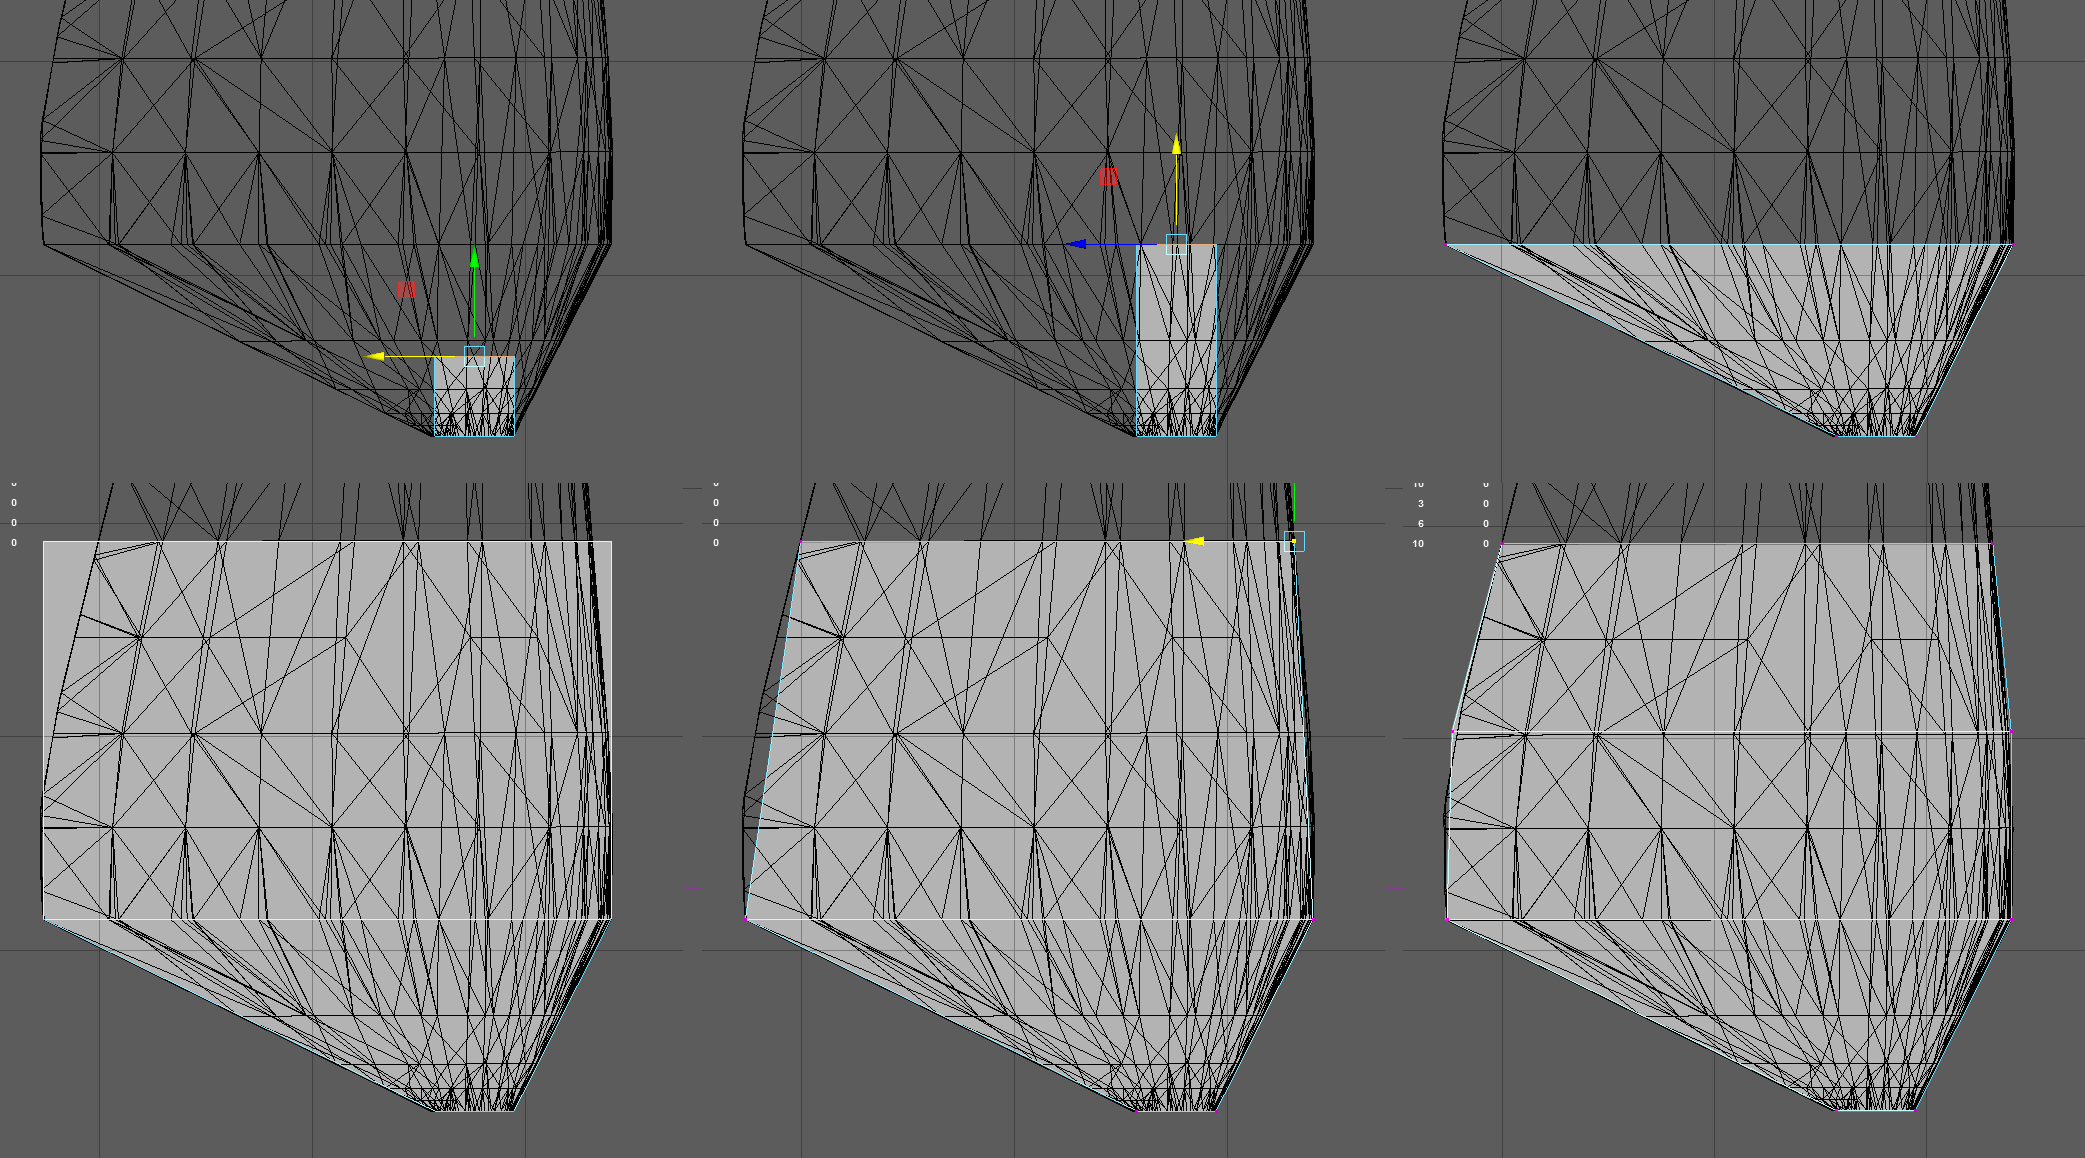
\includegraphics[keepaspectratio, width=1\textwidth]{bildquellen/mod}
	\caption{Retopologisierung einer Teilfläche durch Erzeugung eines Primitives, Anpassung der Vertices, Flächenextrusion und Einsetzen einer weiteren Unterteilung (Edgeloop).}
	\label{fig:2.5}
\end{figure}

Die Gesamte Retopologisierung des CAD-Exportes fand mit mehr oder weniger diesen Werkzeugen statt. Die Abbildung verdeutlicht noch einmal den Unterschied. Das alte Rotorblatt weist eine Anzahl von 1130 Polygonen auf. Das neue Modell setzt sich aus 76 Polygonen zusammen. Es konnten also etwas mehr als 93\% der Flächen eingespart werden \sieheAbb{2.6}. 

\begin{figure}[H]
	\centering
	\captionsetup{width=0.6\textwidth}
	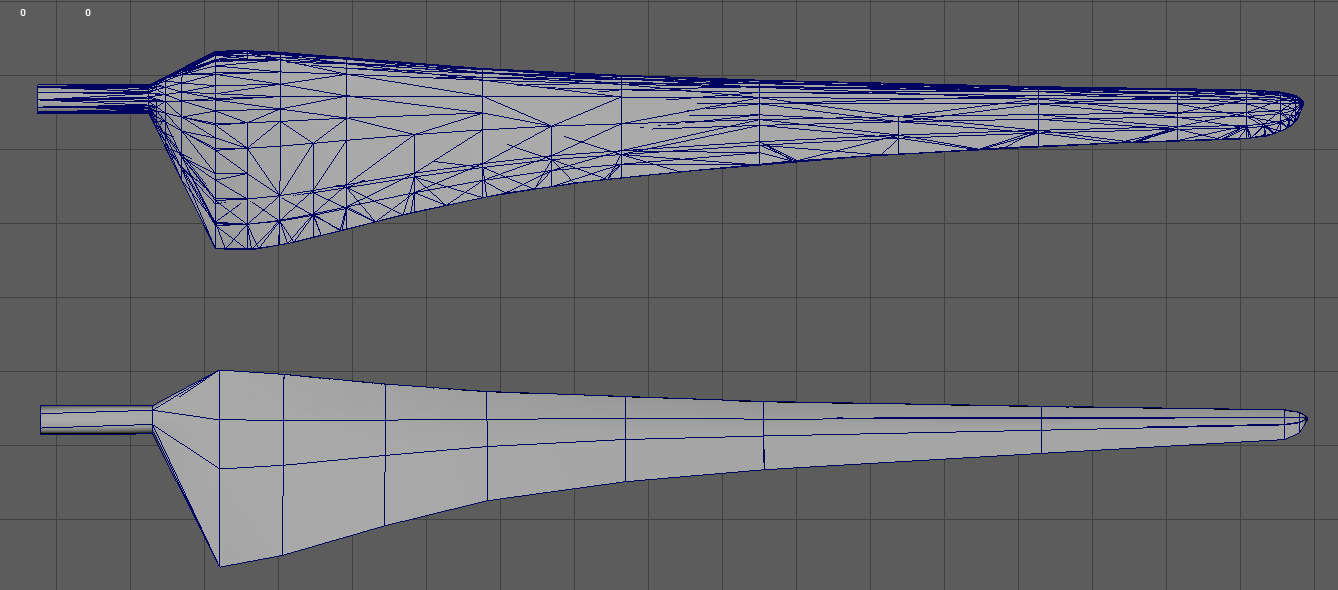
\includegraphics[keepaspectratio, width=0.6\textwidth]{bildquellen/rotorblattGeo}
	\caption{Vergleich des Rotorblattes aus dem CAD-Export (1130 Polygone) mit dem neu erstellten Rotorblatt(76 Polygone).}
	\label{fig:2.6}
\end{figure}

Für ein einzelnes Objekt sind über 1000 Polygone kein Problem. Da es sich bei diesem Rotorblatt aber um eines von vielen Bauteilen handelt, kann die Polygondichte sehr schnell ausufern und die Hardware überfordern. Wenn sich das Objekt mit weniger Polygonen ähnlich gut beschreiben lässt, sollte diese Sparmaßname unbedingt greifen. Zudem gilt natürlich auch hier der Grundsatz des sparsamen Umgangs mit Hardware Ressourcen, wie das generell in der Softwareentwicklung der Fall sein sollte.  

\begin{figure}[H]
	\centering
	\captionsetup{width=1\textwidth}
	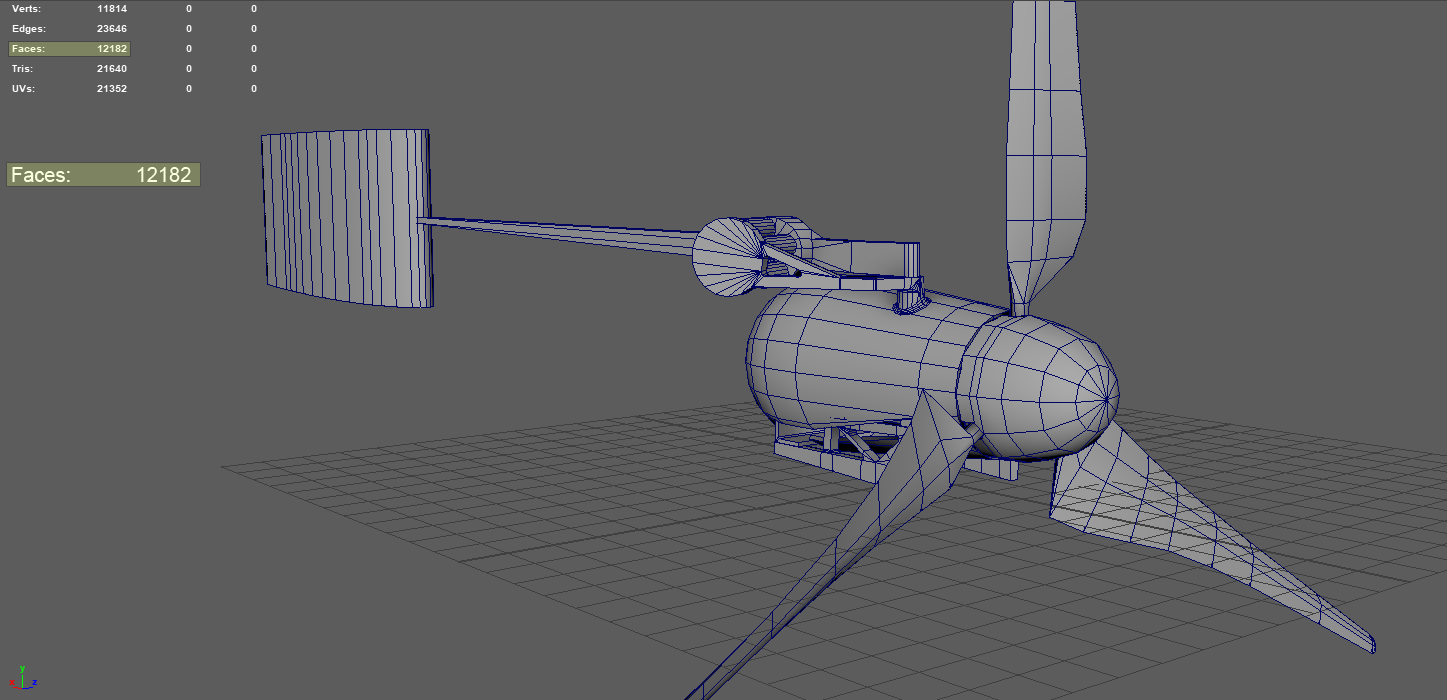
\includegraphics[keepaspectratio, width=1\textwidth]{bildquellen/WEA-Vergleich2}
	\caption{Ergebnis der Retopologisierung bestehend aus 12.182 Polygonen.}
	\label{fig:2.7}
\end{figure}

Das Endergebnis der Retopologisierung kann in der folgenden Abbildung betrachtet werden  \sieheAbb{2.7}. Im Gegensatz zum CAD-Export, der aus 494.988 Polygonen besteht, enthält das neue Modell nur 12.182 Polygone. Es lässt sich konstatieren, dass in Summe ca. 97,5 aller Flächen eingespart wurden.
